\documentclass[journal]{IEEEtran}
\usepackage[brazil, english]{babel}
\usepackage{graphicx}
\usepackage{float}

\begin{document}

\title{Processador de Dois Núcleos}

\author{Gustavo Cruz,
        Otávio Kochi,
        Vinícius Menossi{
\begin{center}
    Universidade Estadual de Maringá - Centro de Tecnologia - Departamento de Informática
\end{center}}
{\begin{center}
    Maringá, 11 de dezembro de 2020
\end{center}}}

\maketitle

\selectlanguage{brazil}
\begin{abstract}
Ao longo dos anos, os processadores evoluíram, e foram sendo criadas arquiteturas multicores que consistem em utilizar de vários núcleos de processamento para executar fluxos concorrentes, assim foi possível construir computadores mais potentes compostos de vários processadores menos potentes. O tema deste trabalho é o simular um processador de dois núcleos em que ambos os núcleos utilizam o Scoreboarding.Neste trabalho serão contempladas como entrada dois programas distintos escritos em MIPS32 os quais serão executados em duas \textit{threads} separadas simulando a execução multinucleada.
\end{abstract}

\begin{IEEEkeywords}
Processador Multinúcleo, Scoreboarding, Artigo, \LaTeX.
\end{IEEEkeywords}

\section{Introdução}

\IEEEPARstart{U}{m} processador é um componente que não se restringe à executar apenas um fluxo de instruções, os arquitetos de computadores têm buscado um projeto de criar computadores poderosos conectando muitos computadores menores, essa visão deu origem ao que se chama multiprocessadores. Atualmente, temos modelos de processadores com cada vez mais núcleos físicos, isso sem citar os núcleos lógicos. Um processado multinúcleo ou multicore possibilita a paralelização do fluxo de execução, ou seja, executar mais de um fluxo ao mesmo tempo. Fluxos de execução, nem sempre são de programas diferentes, e, com o auxílio de bibliotecas especiais, é possível criar programas que funcionem com fluxos de execução distintos, como é o caso da biblioteca \textit{Pthread} da linguagem C. Esta biblioteca possibilita a criação de programas que podem possuir \textit{'n'} fluxos de instruções distintos e estes serão executados de forma paralela pelo processador, usando todos os núcleos disponíveis.

\section{Biblioteca Pthread}
Biblioteca que permite a criação de \textit{threads}, que por sua vez tem como objetivo desenvolver programas paralelos. Essa biblioteca possui funções a fim de controlar tais \textit{threads}, detre as funções podemos destacar as principais: \textit{\textbf{pthread\_create}} utilizada para realizar a criação de uma \textit{thread}; \textit{\textbf{pthread\_join}} utilizada para aguardar a finalização de uma \textit{thread}; \textbf{\textit{pthread\_mutex\_lock, pthread\_mutex\_unlock}} utilizadas garantir que efeitos sobre dados compartilhados sejam equivalentes serialmente, ou seja, uma trava que determina acesso exclusivo aos dados compartilhados para não serem corrompidos.

\section{Implementação}

A implementação deste trabalho foi realizada com o código base do trabalho anterior \textit{Scoreboarding}, sendo realizado alguns ajustes para contemplar o seu objetivo. As alterações realizadas ocorreram em apenas três arquivos: main.c, structs.h e processor.h. No arquivo structs.h foi apenas adicionado uma nova \textit{struct} definida como \textit{thread\_info}, em que tal estrutura possui 6 atributos: id da thread, número da thread, nome do arquivo de configuração, nome do arquivo de saída, nome do programa e a quantidade de instruções que o arquivo do programa possui. As alterações do arquivo processor.h foi realizada da seguinte maneira: Todas as variáveis globais que o arquivo possuía foram convertidas em variáveis locais dentro da função \textit{scoreboardingFunction}, esta alteração foi realizada devido ao uso de \textbf{pthread}, uma vez que com o uso dela, as variáveis globais são compartilhadas entre todas as \textit{threads}, com isso foi optado por alterar o escopo ao invés de utilizar a função \textbf{\textit{lock}}. Com isso foi necessário passar todas essas variáveis como parâmetro de funções que a utilizam. Já no arquivo main.c, as alterações realizadas foram: Adicionar uma nova função \textit{\textbf{core}}, que realiza a chamadas das funções para converter o arquivo de instruções, ler o arquivos de configuração e por fim a função do \textit{scoreboarding}. Foi acrescentado novos parâmetros para a função \textit{getopt} para ser possível pegar os parâmetros de ambos os arquivos. Criada uma variável \textit{tinfo} do tipo \textit{thread\_info}, para armazenar os valores que foram passados através do \textit{getopt}. Também foi adicionado a biblioteca de \textit{pthreads}, para realizar a criação de duas \textit{threads} dentro da função \textit{main}, para isso foi utilizado um laço de repetição utilizando a função \textit{pthread\_create}, onde é a função \textit{core} é passada como parâmetro, bem como as informações das \textit{threads}. Por fim é utilizado também um laço for chamando a função \textit{thread\_joins} para aguardar o fim das \textit{threads} e realizamos um \textit{free} na variável \textit{tinfo}.

\subsection{Arquitetura do Processador Multinúcleo}
\begin{figure}[H]
\caption{Arquitetura Implementada}
\centering
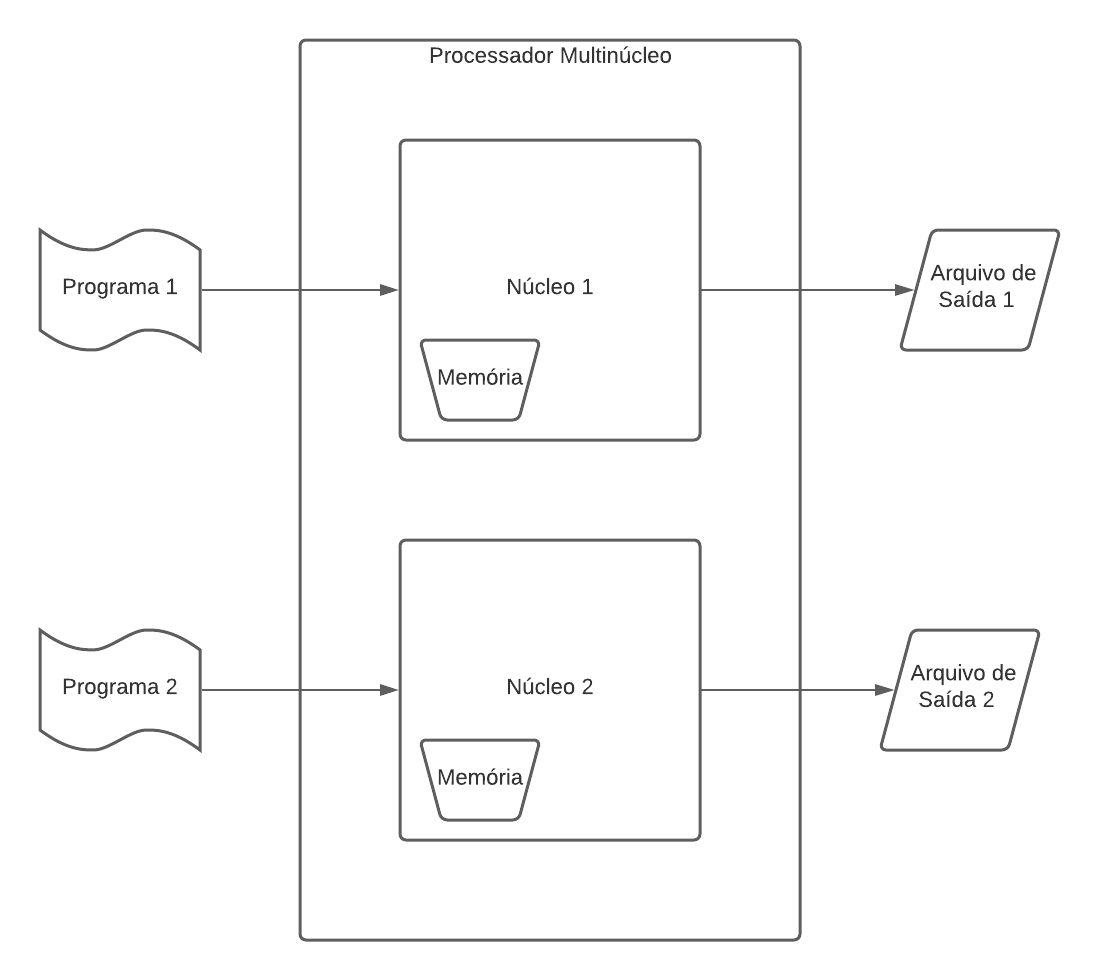
\includegraphics[width=8cm]{ARQ2 - Processador.png}
\end{figure}

A arquitetura feita no simulador implementado segue a ideia de uma execução de dois programas em paralelo, estes possuem, cada um deles, uma memória, uma entrada e uma saída. Cada um dos núcleos implementa um escalonador dinâmico baseado no \textit{Scoreboarding}.

\subsection{Fluxo Interno de um Núcleo}
\begin{figure}[H]
\caption{Fluxo Interno - Busca e Decodificação}
\centering
\includegraphics[width=7cm]{ARQ2 - Núcleo - 1.png}
\end{figure}

O registrador PC é utilizado pela busca para acessar o endereço de memória da instrução atual, a memória devolve a instrução correspondente e então essa e repassada para a unidade de decodificação, que decodifica a instrução para que o processador possa utiliza-la.

\begin{figure}[H]
\caption{Fluxo Interno - Emissão}
\centering
\includegraphics[width=7cm]{ARQ2 - Núcleo - 2.png}
\end{figure}

Na emissão é feita a checagem se a unidade funcional destinada a executar a operação da instrução atual está ocupada, e também é feito a checagem do \textit{hazard write after write} WAW, caso não haja dependências do tipo WAW e haja uma unidade funcional disponível que executa a operação correspondente a instrução atual, então a instrução é emitida.

\begin{figure}[H]
\caption{Fluxo Interno - Leitura}
\centering
\includegraphics[width=7cm]{ARQ2 - Núcleo - 3.png}
\end{figure}

Na leitura, começa o paralelismo do \textit{Scoreboarding}, isso significa que todas as instruções que possam ser lidas, devem ser lidas. Após um controle de concorrência para ver qual pode ser lida e qual não pode, é verificado se a instrução não possui nenhuma dependência, e, caso não tenha, a leitura dos operandos acontece, ou seja, a memória dos registradores é acessada e a instrução com seus valores já resgatados da memória é passado adiante.

\begin{figure}[H]
\caption{Fluxo Interno - Execução}
\centering
\includegraphics[width=7cm]{ARQ2 - Núcleo - 4.png}
\end{figure}

Quando a instrução chega no estado de execução, então é somente ali que a operação realizada pela insturção é executada e seu resultado obtido, cada tipo de operação pode necessitar de diferentes numeros de ciclos de clock para ser executada, após o termino da execução o resultado a ser escrito é enviado a unidade de escrita. 

\begin{figure}[H]
\caption{Fluxo Interno - Escrita}
\centering
\includegraphics[width=7cm]{ARQ2 - Núcleo - 5.png}
\end{figure}

Na última parte do fluxo interno temos a Escrita. Primeiramente é feito uma verificação de quais são as instruções que podem ser escritas e se não existir nenhuma dependência do tipo \textit{WAR}, a escrita pode ser realizada, ou seja, a memória dos registradores pode ser alterada. Além disso, todas as unidades funcionais que desocuparam devem sem atualizadas, removendo quaiquer informações contidas lá dentro.

\begin{thebibliography}{}
\bibitem{} 
PATTERSON, David A.; HENNESSY, John L.. Computer Architecture, Fifth Edition: A Quantitative Approach. 5. ed. 2011.

\bibitem{}
STALINGS, William. Computer Organization and Architecture: design for performance. 4. ed. Pearson, 1987.



\end{thebibliography}

\end{document}